\documentclass{article}
\usepackage[utf8]{inputenc}
\usepackage{graphicx}

\title{Principal Component Analysis}
\author{Diego Brunetto da Silva,\\Pedro Henrique Levy Fermino Ferreira}

\date{07.12.2022}

\begin{document}

\maketitle
\section{Encontrando um Dataset...}
\par
Aqui vamos discorrer a respeito do que é nosso dataset, e como o acessamos.
\subsection{Importando o Dataset...}
\par
Importamos então a base de dados, que estava em Excel ao extrair:
\begin{verbatim}
    pb = pd.read_excel()
\end{verbatim}
\subsection{Tratando os dados...}
\par
Utilizamos o comando 'describe' para ter acesso a informações estatísticas dos dados, utilizamos o comando 'mean' para então subtrair do total a média, normalizando assim os dados.
\begin{verbatim}
pb.describe()
mean = np.mean(pb,axis=0)
Reducepb = pb - mean
-> Reducepb
\end{verbatim}
\section{Calculando a Covariância...}
\par
Foi feito então, o cálculo da matriz de Covariância, a partir dos comandos:
\begin{verbatim}
    Covariância_da_Matriz = np.cov(Reducepb)
    -> Covariância_da_Matriz	
\end{verbatim}
\section{Calculando os autovalores e autovetores...}
\par
Para tal, foi utilizado o comando:
\begin{verbatim}
    autovalores, autovetores = np.linalg.eig((Covariância_da_Matriz))
np.sum(autovalores)
\end{verbatim}
\section{Escolhendo os 2 maiores autovalores...}
Definiu-se o 'Dataframe' (df):
\begin{verbatim}
    df = pd.DataFrame(pb)
\end{verbatim}
E então, foi feita e plotada a seleção dos dois maiores autovalores:
\begin{verbatim}
    selection = df[['Belgium','Malta' ]]
    -> selection
\end{verbatim}
\section{Plotando o gráfico}
Por fim, plotamos o gráfico de linhas que representava as colunas dos dois maiores autovalores:
\begin{verbatim}
    sbs.lineplot(x="Belgium", y="Cyprus",data = pb)
plt.show()
\end{verbatim}
\hline
\section{Gráfico}
\begin{figure}
    \centering
    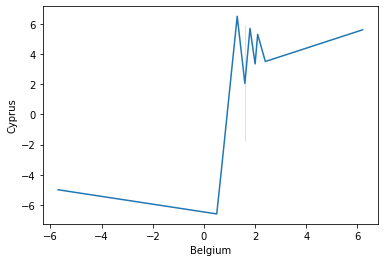
\includegraphics{figs/graphic.png}
    \caption{Plot das duas colunas correspondentes}
    \label{fig:my_label}
\end{figure}
\end{document}
